

در آزمایش ششم امکان ذخیره‌سازی در 
\lr{RAM}
و همچنین
امکان پرش در دستورات را نداشتیم.
در این آزمایش این قابلیت‌ها به مدار اضافه می‌شوند
و همچنین دو برنامه با استفاده  از آن‌ها می‌نویسیم.

در ابتدا ماژول 
\lr{RAM}
را به برنامه اضافه می‌کنیم و برای این منظور از 
چهار عدد 
\lr{7489}
استفاده می‌کنیم که یک 
\lr{RAM}
با 
$16$
حافظه‌ی
$4$
بیتی است.
با استفاده از 
این قطعه به صورت
\lr{submodular}
قطعه 
\lr{RAM}
را همانند شکل زیر طراحی می‌کنیم.

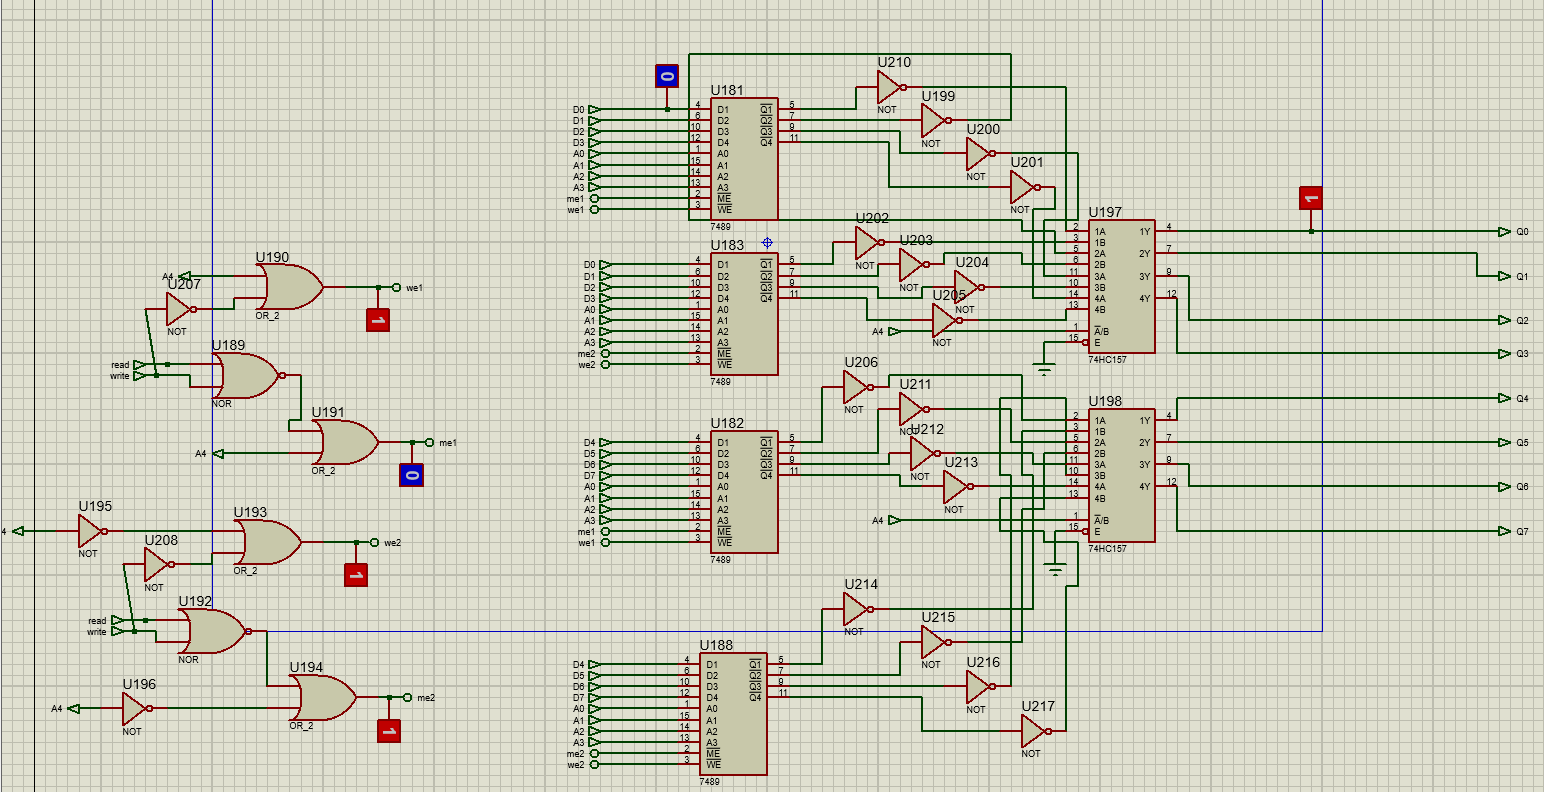
\includegraphics[width=18cm]{figures/RAM.png}

که از دو قطعه‌ی 
\lr{75157}
هم به عنوان مولتی‌پلکسر در این طراحی استفاده شده است.

در ادامه با استفاده از دو
\lr{4 bit adder}
به صورت
\lr{submodular}
یک قطعه‌ی
\lr{8 bit adder}
به صورت زیر طراحی می‌کنیم.

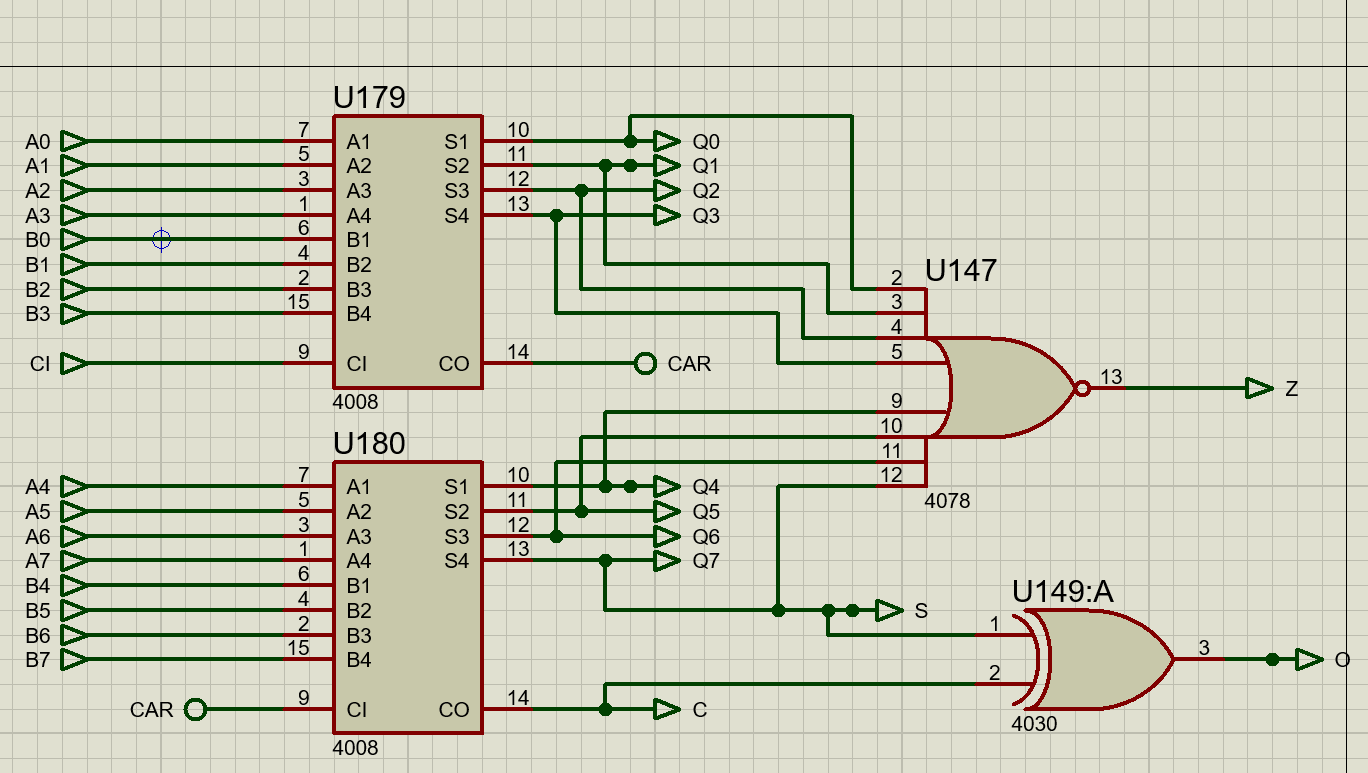
\includegraphics[width=18cm]{figures/Adder.png}

در این قطعه
$4$
پرچم
\lr{overflow}
،
\lr{carry}
،
\lr{sign}
و
\lr{zero}
نیز همانند تصویر بالا طراحی شده‌اند.

در ادامه ماژول
\lr{program counter}
را طراحی می‌کنیم که همانند
یک
\lr{counter}
است که قابلیت 
\lr{load}
هم دارد.
برای زیاد کردن 
\lr{PC}
به مقدار یک واحد و یا
استفاده از
\lr{branch}
این قابلیت‌ها مورد نیازمان می‌شود.
همانند شکل زیر این قطعه را کامل می‌کنیم.
این مدار علاوه بر کلاک های هر بخش و سیگنال های ریست، وظیفه تعیین عملیات  ALUرا نیز بر عهده دارد


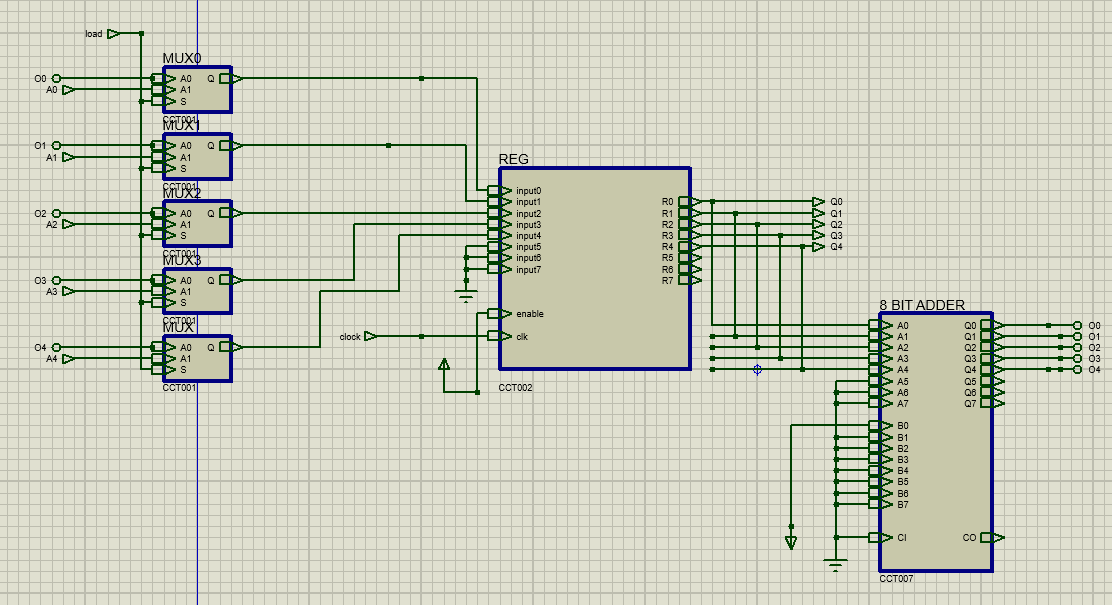
\includegraphics[width=18cm]{figures/PC.png}

\pagebreak 

در ادامه ماژول
\lr{controll unit}
را طراحی می‌کنیم
که پایه‌های کنترلی مدارمان را کنترل می‌کند
طراحی این مدار به شکل زیر خواهد بود.

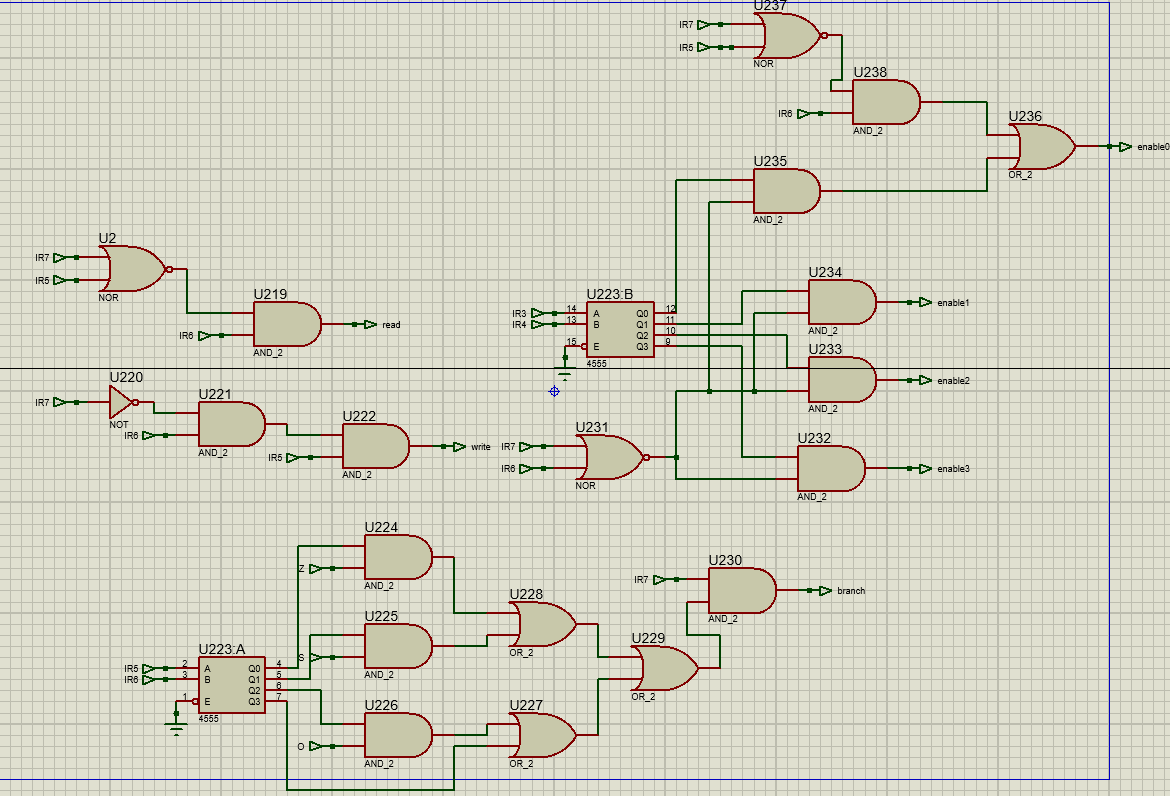
\includegraphics[width=18cm]{figures/CU.png}

در نهایت با متصل کردن تمام ماژول‌هایی که طراحی کردیم مدار نهایی به شکل
زیر خواهد بود.

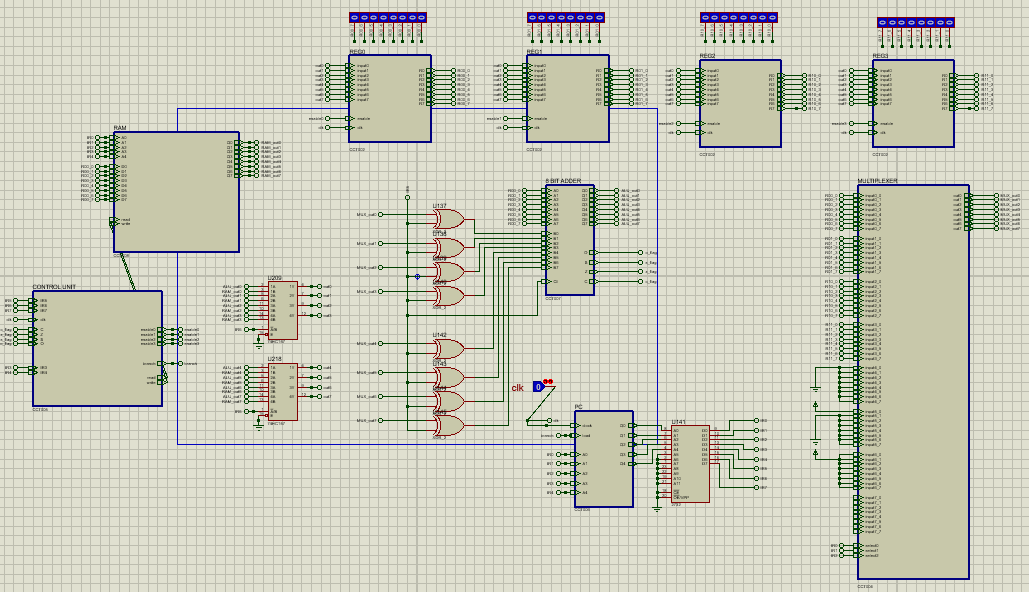
\includegraphics[width=18cm]{figures/all.png}

\pagebreak

در ادامه از ما خواسته شده است 
تا برنامه
\lr{fibonnaci}
را با این زبان بنویسیم و
با توجه به مداری که طراحی کردیم 
\lr{hex code}
زیر را برای آن طراحی می‌کنیم که
در نهایت جمع
$5$
جمله اول فیبوناچی داخل رجیستر اول قرار می‌گیرد.

\raggedright

$200C0512090112090112200260ED$

\raggedleft

که درنهایت با اجرا کردن آن خروجی زیر را خواهیم گرفت که به درستی
جمع
$5$
جمله‌ی اول فیبوناچی که
$12$
است را محاسبه می‌کند.


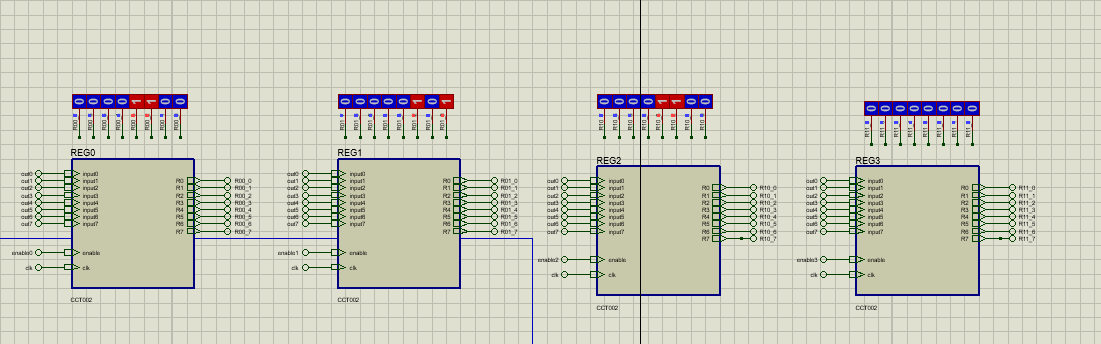
\includegraphics[width=18cm]{figures/fib.png}
و در نهایت
تمام قسمت‌های این گزارش
اعم از فایل
های برنامه
\lr{hex}
و 
پروژه‌ی
\lr{proteus}
در پیوست قرار داده شده‌اند.





